\chapter{Metodologia}
%\chapter{Conjunto de Dados e Questões de Pesquisa}
\label{cap:qp}

Este trabalho propõe um estudo sobre as \textit{breaking changes} em \textit{releases minor} e \textit{patch} e seus impactos no ecossistema do \textsf{npm}. Para isso, três questões de pesquisa foram elaboradas para direcionar nosso estudo. Apresentamos a seguir os procedimentos para a coleta de dados e as motivações e os métodos de cada uma dessas questões de pesquisa.

\section{Coleta do Conjunto de Dados}
\label{sec:col_base}
O conjunto de dados utilizado neste trabalho foi extraído do registro do \textsf{npm}, do qual foram recuperados os arquivos de metadados \textit{package.json} de 1,233,944 pacotes publicados no período de 20 de Dezembro de 2010 até 01 de Abril de 2020. Os principais dados recuperados no \textit{package.json} são os \textit{timestamp} de cada uma das \textit{releases} dos pacotes, os provedores que os pacotes clientes continham em cada \textit{release} e suas respectivas versões. A Figura \ref{fig:package_json} exibe as informações do pacote \textsf{buffer-includes}\footnote{http://registry.npmjs.org/buffer-includes} que podem ser recuperadas de seu \textit{package.json}.

\begin{figure}
    \centering
    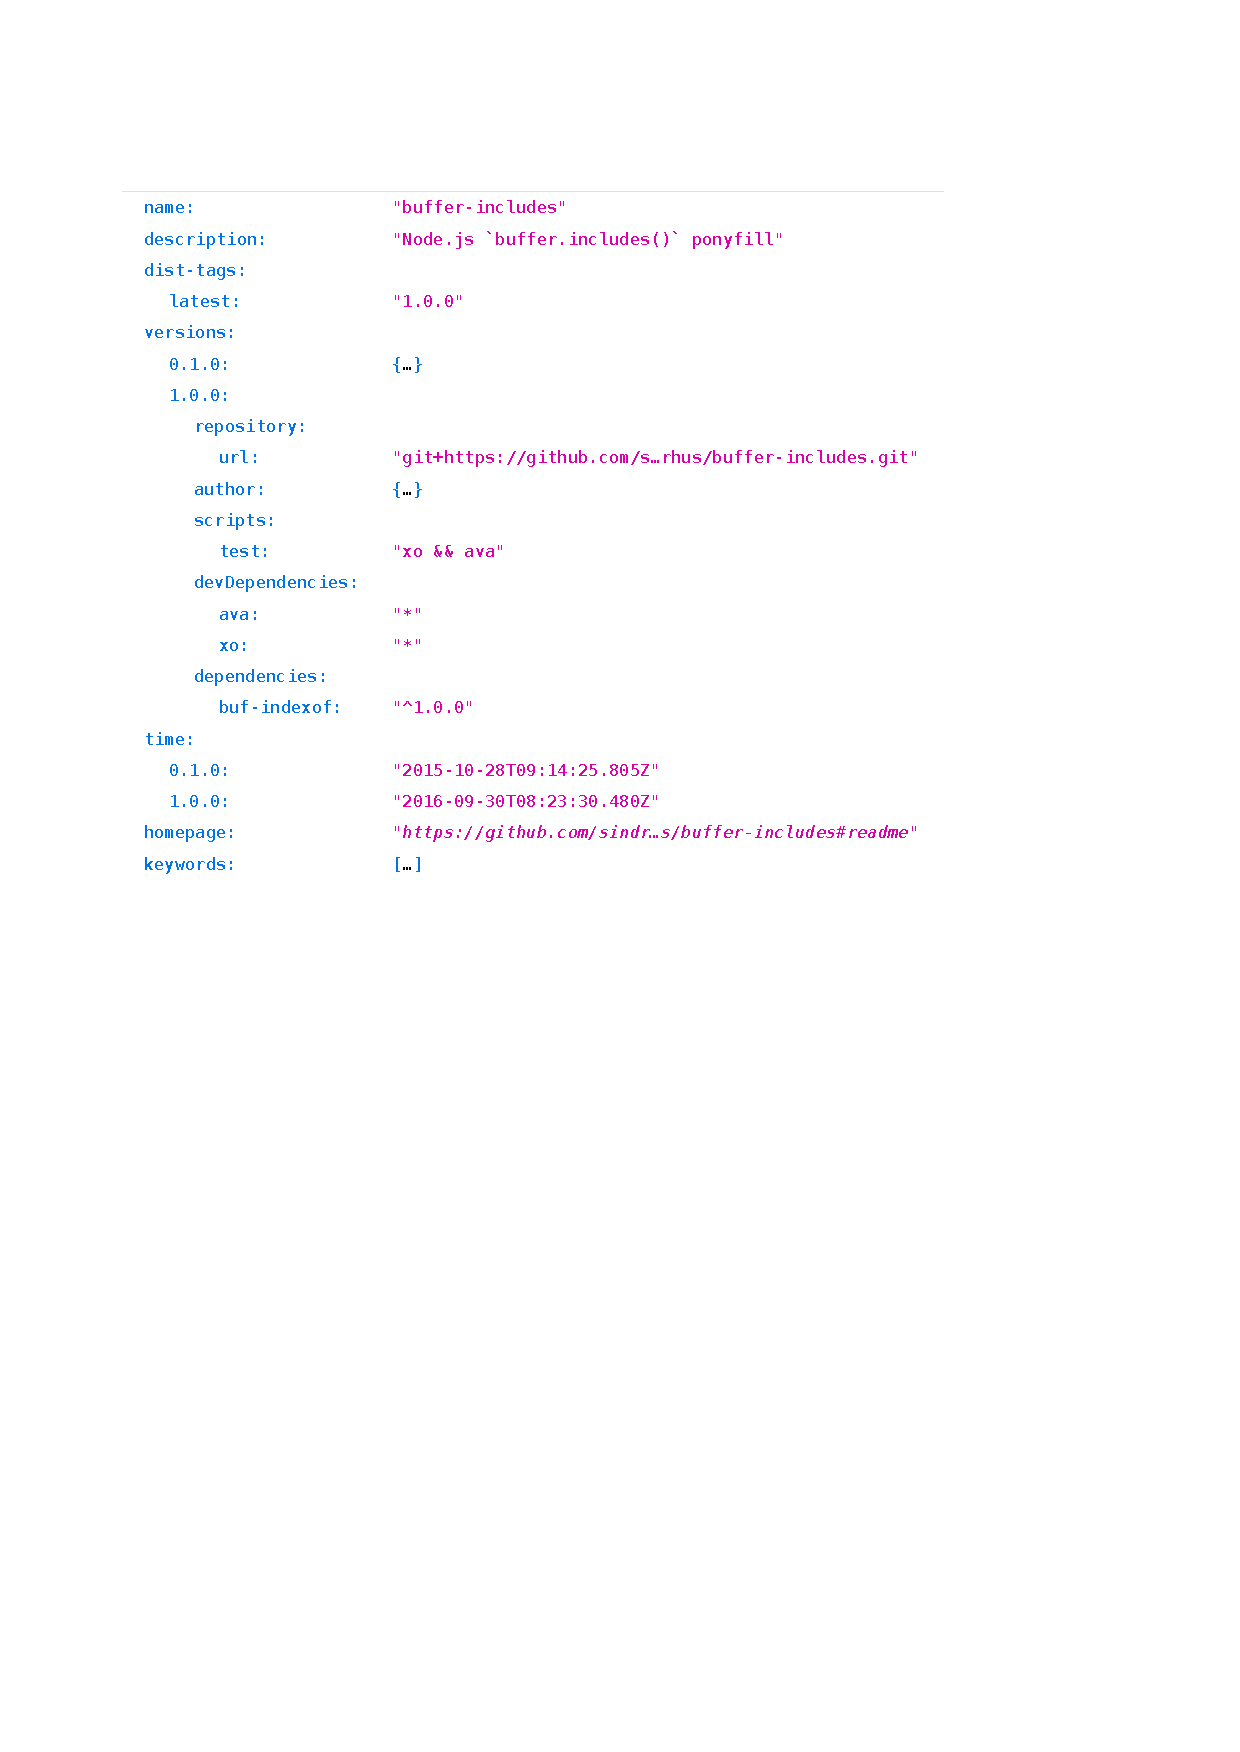
\includegraphics[scale=0.65]{figuras/package_json.pdf}
    \caption{Informações que serão recuperadas do \textit{package.json} para validar um pacote.}
    \label{fig:package_json}
\end{figure}{}

Foram excluídos desse conjunto de dados todos os pacotes que não continham nenhum provedor, pois quando um pacote não contém provedores não há como ser impactado por \textit{breaking changes}. Dessa maneira, o conjunto de dados final foi reduzido para um total de 987,595 pacotes clientes do \textsf{npm}. Por fim, para cada \textit{release} de todos os clientes, foram resolvidas as versões de todos os provedores com base no \textit{timestamp} dessa \textit{release}. Ou seja, foi resolvido o \textit{range} do provedor, que o cliente especificou naquela \textit{release}, para a maior versão aceita no momento da \textit{release} do cliente. Desse modo, foi determinada qual a versão do provedor o cliente utilizava no momento da publicação da \textit{release}.

\section{Amostra do Conjunto de Dados}
\label{sec:col_amostra}
% para remover a lista de siglas, foi utilizado um \textit no http
Para gerar a amostra utilizada neste trabalho, foram verificados dois requisitos nos \textit{987k} pacotes clientes: 1) possuir um \textit{script} de teste não vazio e diferente do \textit{script} padrão de teste do \textsf{npm}: \texttt{\{"test": "Error: no test specified"\}} (488,805 conferem); e possuir a \textit{url} do repositório (410,433 conferem). Esses dois requisitos foram analisados na última \textit{release} disponível do pacote. Então, foi recuperada uma amostra representativa com 95\% de confiança e 5\% de margem de erro. Dentre os 410,433 pacotes clientes restantes, a amostra resultou em 384 pacotes para serem analisados neste trabalho.

Foi realizada uma verificação manual nos repositórios do pacotes com menos de 4 \textit{releases} (130 dentre 384) para verificar se cada pacote não era um \textit{toy package}, ou seja, um pacote que não foi criado para ser um projeto real, apenas um teste no \textsf{npm}, no \textsf{GitHub} ou algo do tipo. Um pacote foi classificado como \textit{toy package} e substituído por outro que foi sorteado seguindo os dois requisitos leçãopara se.

\section{Metodologia para Detecção de \textit{Breaking Changes}}
\label{sec:bcdetect}
Para este trabalho, desenvolvemos uma ferramenta chamada \textsf{BCDetect}\footnote{https://github.com/danielventurini/bcdetect} disponível no \textsf{GitHub} sob a licença \textsf{MIT}. Esta ferramenta clona o repositório do respectivo cliente -- todos os clientes estavam hospedados no \textsf{Github} -- e cria uma estrutura de dados para armazenar as informações sobre o cliente. Nessa estrutura, cada \textit{release} do cliente contém todos os provedores com suas versões resolvidas e o tipo de atualização que os provedores realizaram desde a última \textit{release} do cliente: \texttt{steady} significa que o provedor não publicou nenhuma \textit{release} aceita desde a última release do cliente; \texttt{upgrade} significa que o provedor publicou uma nova \textit{release} aceita desde a última \textit{release} do cliente; e quando não há nenhuma dessas informações, o provedor foi inserido no \textit{package.json} nesta \textit{release}. Essa estrutura básica está representada na Figura \ref{fig:bc_work}, construída a partir dos dados do cliente \textsf{buffer-includes} da Figura \ref{fig:package_json}.

\begin{figure}
    \centering
    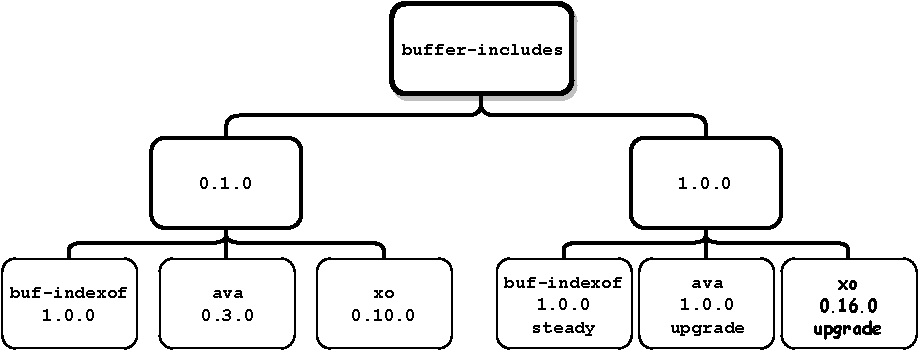
\includegraphics[scale=0.9]{figuras/bcdetect_work.pdf}
    \caption{Estrutura de dados para representar o cliente \textsf{buffer-includes}.}
    \label{fig:bc_work}
\end{figure}{}

Os testes de cada \textit{release} do cliente foram executados toda vez que havia pelo menos um provedor com uma nova \textit{release} (\textit{upgrade}) ou um provedor havia sido adicionado naquela \textit{release} do cliente. Após clonado o repositório, foi executado o comando \texttt{git checkout} para todas as \textit{releases} do cliente -- \textit{release} por \textit{release} -- com a respectiva \textit{tag} da \textit{release}, fazendo com que todos os arquivos sejam restaurados para exatamente os mesmos arquivos do momento em que o cliente publicou a \textit{release}. Uma \textit{tag} é uma referência a um ponto importante e específico do repositório, que geralmente são as \textit{releases}. Para \textit{releases} que o desenvolvedor não criou uma \textit{tag}, o \textit{checkout} foi realizado usando o \textit{timestamp} da respectiva \textit{release}. Em seguida, o arquivo \textit{package-lock.json}\footnote{https://docs.npmjs.com/files/package-lock.json} foi excluído, pois esse arquivo altera o comportamento do comando \texttt{npm install} -- a partir do \textsf{npm@5} -- fazendo com que o \textsf{npm} instale as versões dos provedores de acordo com o \textit{package-lock.json}, e não de acordo com o \textit{package.json}. Em sequência, todos provedores no \textit{package.json} e suas respectivas versões foram adicionados apenas no campo \textit{dependencies} do \textit{package.json} e os demais campos foram removidos,\footnote{campos para dependências no \textit{package.json}, tais como o \textit{peerDependencies}, \textit{optionalDependencies} e o \textit{globalDependencies}} uma vez que para executar os testes, ambos os provedores são requeridos.

O \textsf{Node.js} é o ambiente de execução para os pacotes \textsf{JavaScript} e a cada 6 meses uma nova \textit{release major} é publicada.\footnote{https://github.com/nodejs/node\#release-types} Por isso, antes de executar os testes da \textit{release} do cliente, a versão do \textsf{Node.js} precisa ser alterada. O chaveamento das \textit{releases} do \textsf{Node.js} é necessário pois as \textit{releases major} do \textsf{Node.js} não são retrocompatíveis, ou seja, um pacote que executa com sucesso na versão \textit{0.x} do \textsf{Node.js}, por exemplo, provavelmente não executaria com sucesso na versão \textit{8.x}. Para cada \textit{release} do cliente que teria seus testes executados, a versão do \textsf{Node.js} foi selecionada de duas maneiras: 1) do campo \texttt{engines->node} no \textit{package.json}, que permite o desenvolvedor especificar a versão do \textsf{Node.js}; e 2) através do \textit{timestamp} da \textit{release} do cliente, foi possível identificar a última \textit{release} do \textsf{Node.js} disponível,\footnote{https://nodejs.org/en/download/releases} ou seja, qual era a \textit{release} máxima do \textsf{Node.js} que os testes dos cliente foram executados no momento da \textit{release} do cliente. Assim, os testes do cliente foram executados em todas as versões \textit{major} do \textsf{Node.js}, da versão mais atual, pelo \textit{timestamp} da \textit{release} do cliente, até a versão \textit{major} mais antiga, ou até o teste executar com sucesso. Para o cliente da Figura \ref{fig:bc_work}, a sua \textit{release 0.1.0} possui o \textit{timestamp} como \textit{2015-10-28}, e a última \textit{release} do \textsf{Node.js} disponível até esta data é a \textit{4.2.1}. Assim, os testes dessa \textit{release} do cliente seriam executados com as \textit{releases 4.x, 3.x, 2.x, 1.x, 0.x} do \textsf{Node.js}. Ao atualizar a \textit{release} do \textsf{Node.js}, a versão do \textsf{npm} é atualizada também. Isso é necessário pois é o \textsf{npm} que executa os \textit{scripts install} e \textit{test}. Após executar o \textit{install} e o \textit{test}, foram salvas as seguintes informações:

\begin{itemize}
    \item versão do cliente;
    \item se houve alteração na versão aceita de alguns dos provedores;
    \item os códigos da execução do \texttt{npm install} e \texttt{npm test} -- sucesso ou erro;
    \item a versão do \textsf{Node.js} que deveria ser executado com base na data da \textit{release}; e
    \item a versão do \textsf{Node.js} que os testes do cliente executaram com sucesso.
\end{itemize}{}

Os passos resumidos das operações em cada cliente juntamente com a verificação de alteração dos provedores e execução dos testes das \textit{releases} se encontram na Figura \ref{fig:steps_work}.

\begin{figure}
    \centering
    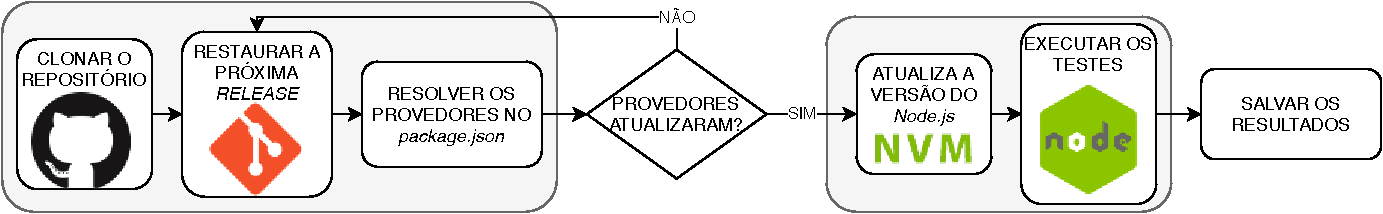
\includegraphics[scale=0.7]{figuras/steps_work.pdf}
    \caption{Etapas para clonar, restaurar e execução os testes das \textit{releases} de um cliente}
    \label{fig:steps_work}
\end{figure}{}

Dos 384 clientes que tiveram seus testes executados, em 33 não foi possível executar o comando \texttt{npm install}/\texttt{test} para nenhuma de suas \textit{releases}. Desses 33 clientes, 15 não possuíam algum dos arquivos necessários para os testes; 11 continham \textit{scripts} de teste inválidos em todas as suas \textit{releases}, tal como \texttt{\{"test": "no tests"\}}; 4 haviam listados alguns dos arquivos no \textit{.gitignore} -- arquivo utilizado pelo \textsf{git} para ignorar arquivos no repositório --, mas que eram necessários para a execução dos testes; 2 necessitaram de configurações específicas em banco de dados e não foi possível realizá-las; e 1 cliente requeria uma variável de ambiente para acessar um determinado site. Dessa forma, os 33 clientes foram substituídos em um novo sorteio seguindo o mesmo critério do sorteio anterior citado na Seção \ref{sec:col_amostra}, totalizando 384 clientes com 5957 \textit{releases} que foram utilizados no estudo.

Um pacote de replicação incluindo a amostra utilizada neste trabalho, as ferramentas, \textit{scripts} e todos os casos de \textit{breaking changes} está disponível no \textit{Zenodo}.\footnote{https://doi.org/10.5281/zenodo.4284035}

%---------------------------------------------------%
%----------------------RQ1--------------------------%
%---------------------------------------------------%

\section{Questões de Pesquisa}

Apresentamos nessa seção as questões que norteiam nossa pesquisa e investigação.

\subsubsection{\large QP1. Com que frequência \textit{breaking changes} impactam os clientes?}
\label{sec:qp1}

% \subsubsection{Motivação:}
% \label{sec:qp1:motivation}
\textbf{Motivação:}
no ecossistema do \textsf{npm}, uma \textit{release} que contenha um erro pode afetar uma grande quantidade de pacotes, uma vez que a rede de dependências do \textsf{npm} é relativamente densa \cite{teorical_reference:npm_2}. Para evitar que \textit{breaking changes} se manifestem nos clientes, os provedores introduzem as \textit{breaking changes} em \textit{releases major}, seguindo o padrão do Versionamento Semântico, e os clientes podem utilizar \textit{strings SemVer} para aceitar apenas as versões \textit{minor} e \textit{patch} dos provedores -- o padrão do \textsf{npm}. Entretanto, nem sempre o provedor é capaz de distinguir se suas alterações são ou não \textit{breaking changes} \cite{noregrets2018}, e muitas vezes as \textit{breaking changes} são introduzidas sem que os provedores percebam. Estudos anteriores têm abordado \textit{breaking changes} no ecossistema do \textsf{npm} \cite{using_others_tests, noregrets2018, intro:break_change, teorical_reference:bc_1}, mas não estudaram a frequência e como se manifestam. Nesta QP, serão quantificadas as manifestações das \textit{breaking changes} nos clientes.
\newline

% \subsubsection{Método:}
% \label{sec:qp1:approach}
\noindent
\textbf{Método:}
Quando os comandos \texttt{npm install} e \texttt{npm test} resultaram em erro, o nosso objetivo foi distinguir se o erro foi causado pelo provedor, caracterizando uma \textit{breaking change}, ou se foi causado apenas pelo próprio cliente, não sendo uma \textit{breaking change}. A primeira evidência é o \textit{stack trace} gerado pelo \textsf{npm} quando ocorre um erro. O \textit{stack trace} contém o tipo do erro, a localização exata do erro e o fluxo de execução no momento em que o erro ocorreu. Uma das principais informações são os provedores que estavam sendo executados no fluxo de execução. Se houve algum provedor no \textit{stack trace}, provavelmente o erro se tratava de uma \textit{breaking change}. Quando não houve algum provedor no \textit{stack trace}, provavelmente o erro não se tratava de uma \textit{breaking change}, mas ainda sim foram feitos os métodos descritos abaixo para confirmar se um erro era de fato uma \textit{breaking change} ou não.

Para quantificar as \textit{breaking changes}, foi necessário diferenciar entre um erro causado pelo próprio cliente, no qual não houve influência de nenhum provedor, e um erro causado por algum dos provedores, sendo assim uma \textit{breaking change}. Para realizar esta diferenciação, foram realizadas as seguintes heurísticas:

\begin{itemize}
    \item \textbf{Alterações nos códigos}: foram realizadas algumas alterações nos códigos do cliente e do provedor para analisar o fluxo de execução até gerar o erro. Por exemplo, foram adicionadas chamadas para \texttt{console.trace()} para visualizar a pilha de execução até essa chamada. Também, a chamada para \texttt{console.log()} foi muito utilizada para verificar o conteúdo das variáveis em tempo de execução e suas tipagens. Isso tudo para verificar como as variáveis estavam se comportando e como estavam sendo alteradas pelos provedores e pelo próprio cliente.

    \item \textbf{Integração contínua ao \textsf{GitHub}:} sistemas de integração contínua\footnote{https://strongloop.com/strongblog/node-js-travis-circle-
codeship-compare/} são sistemas que integram-se aos repositórios e disponibilizam tarefas automáticas para os desenvolvedores, tal como execução de testes. Essas integrações contínua desempenharam um papel fundamental na análise manual. Se o \textit{status} do teste do \textit{commit} da \textit{release} do cliente nesses sistemas integrados estava como sucesso e em nosso estudo foi identificado como um erro, provavelmente o erro se tratava de uma \textit{breaking change}. Isso pois o \textit{commit} da \textit{release} do cliente no sistema integrado era o mesmo \textit{commit} executado em nosso estudo. Assim, apenas a versão dos provedores poderia ter sido alterada e causado o erro.

    \item \textbf{\textit{Commits} do cliente:} foram analisados manualmente os \textit{commits} do cliente a partir do \textit{commit} da \textit{release} para verificar se o cliente tentou consertar algo em seu código. Se sim, foram realizadas as alterações feitas pelo cliente para verificar se o erro foi consertado e concluir se o erro foi causado apenas pelo pacote cliente ou se foi causado por um dos pacotes provedores. Por exemplo, se um cliente atualizou um provedor e foi impactado por uma \textit{breaking change}, nos próximos \textit{commits} o cliente poderia realizar um \textit{downgrade} na versão do provedor ou realizar uma alteração em seu código para se recuperar da \textit{breaking change}. Os \textit{commits} nomeadas como \textit{"downgrade provider"}, \textit{"fix break change"}, \textit{"Bump tests and dependencies"} indicam que o cliente realizou alguma alteração para, provavelmente, se recuperar da \textit{breaking change}.

    \item \textbf{\textit{Issues/Pull-requests}:} se o erro é uma \textit{breaking change}, outros clientes podem ter sido impactados e provavelmente já foi documentada em uma \textit{issue} ou um \textit{pull-request}. Através dos comentários das \textit{issues}/\textit{pull-requests} foi possível recuperar informações detalhadas sobre o erro, qual provedor introduziu e se foi consertada. \textit{Issues} e \textit{pull-requests} foram muito importantes e permitiram encontrar muitas informações, porque muitas \textit{issues} e \textit{pull-requests} referenciam outras, no mesmo projeto ou em projetos distintos, enquanto os desenvolvedores estão rastreando um erro \cite{Zhang:2018:WIL:3242887.3242891}.

    \item \textbf{\textit{Releases} precedentes e posteriores do provedor:} essa foi uma etapa muito importante para detectar se um erro era uma \textit{breaking change}. Se um erro é uma \textit{breaking change}, as \textit{releases} precedentes e posteriores do provedor poderiam consertar o erro. Nesse caso, foi desinstalada a \textit{release} atual e instalada uma \textit{release} anterior ou posterior àquela que causou o erro. Por fim, o \textit{script} de teste foi reexecutado. Por exemplo, se um cliente especificou um provedor \texttt{p} como \texttt{\{"p": "\textasciicircum1.0.2"\}} e esse provedor introduziu uma \textit{breaking change} na \textit{release}, por exemplo, \texttt{1.0.4}. Então foram instaladas as releases \texttt{p@1.0.2}, \texttt{p@1.0.3} e \texttt{p@1.0.5} para verificar se alguma dessas \textit{releases} não introduziu ou consertou a \textit{breaking change}. Assim, foi possível confirmar em qual \textit{release} do provedor a \textit{breaking change} foi introduzida/consertada.
\end{itemize}{}

Para todos os casos de erro confirmados como \textit{breaking changes}, foram coletadas a data das \textit{releases} dos provedores que introduziram as \textit{breaking changes} para realizar uma análise temporal. O registro do \textsf{npm} está funcional desde 2010 e foi analisada a evolução das \textit{breaking changes} ao longo do tempo.

Para entender quais características as \textit{releases} com \textit{breaking changes} diferem das demais \textit{releases} sem \textit{breaking changes}, foi recuperada, para cada \textit{release} que introduziu a \textit{breaking change}, a quantidade de \textit{commits} que o provedor introduziu em todas as \textit{release} pertencentes ao mesmo nível \textit{major}. Por exemplo, para uma \textit{breaking change} introduzida no provedor \textsf{p@2.0.3}, foi recuperado a quantidade de \textit{commits} introduzida no \textit{range}  \textsf{p@2.x.y}, ou seja, \textsf{p@2.0.0}, \textsf{p@2.0.1}, \textsf{p@2.0.2}, \textsf{p@2.0.3} e assim por diante. Então, foi calculada a mediana dos \textit{commits} introduzidos em cada \textit{release} nesse \textit{range major} para verificar se a \textit{breaking change} na \textit{release} do provedor foi influenciada pela quantidade de \textit{commits}. Entretanto, três provedores foram removidos desta análise pois os seus repositórios são compartilhados com outros pacotes, o que tornou inviável a análise dessa quantidade de \textit{commits} entre duas \textit{releases}, uma vez que seria analisado \textit{commits} dos outros pacotes também. Esses provedores são \textsf{@types/node}, \textsf{@types/lodash} e \textsf{babel-preset-es2015}.

%---------------------------------------------------%
%----------------------RQ2--------------------------%
%---------------------------------------------------%

\subsubsection{\large QP2. Como os provedores introduzem \textit{breaking changes} em uma \textit{release}?}
\label{sec:qp2}

% \subsubsection{Motivação:}
% \label{sec:qp2:motivation}
\textbf{Motivação:}
Pesquisas anteriores apresentam estudos sobre \textit{breaking changes} no ecossistema do \textsf{npm}. Entretanto, pelo fato do \textit{Javascript} ser dinâmico, esses estudos focaram apenas nas alterações de \textit{APIs}, tais como as remoções/renomeações, alterações na lista de parâmetros e alterações no tipo de retorno. Esses estudos foram realizados por  \citeonline{teorical_reference:bc_1} e \citeonline{noregrets2018} e não verificaram \textit{breaking changes} além das relacionadas às \textit{APIs}. Porém, podem haver outros tipos de \textit{breaking changes} no ecossistema do \textsf{npm} além das alterações em \textit{API}. Por causa da falta de informação, muitas \textit{breaking changes} introduzidas poderiam ser facilmente evitadas. Por isso, categorizar as \textit{breaking changes} ajudará os desenvolvedores a atentar-se para as \textit{breaking changes} mais comuns, assim produzindo códigos menos favoráveis a ocorrência das mesmas.
\newline

\noindent
% \subsubsection{Método:}
% \label{sec:qp2:approach}
\textbf{Método:}
O objetivo da análise manual é descobrir o motivo que originou uma \textit{breaking change}, ou seja, qual foi a alteração que o provedor realizou e que causou a \textit{breaking change}, para que seja possível agrupa-las por suas similaridades. Após descobrir em qual versão do provedor a \textit{breaking change} foi introduzida, foi realizada uma análise manual no repositório do provedor para descobrir a exata alteração no código que originou a \textit{breaking change}. As seguintes técnicas foram usadas:

\begin{itemize}
    \item \textbf{Arquivos de alterações:} os arquivos de registros de alterações, comumente nomeados por \textit{CHANGELOG.md} ou \textit{HISTORY.md}, contêm as descrições das principais alterações em cada \textit{releases} do projeto. Uma das informações mais relevantes nestes arquivos são as descrições de \textit{breaking changes}. Por exemplo, a versão \textit{5.0.0} do pacote \textsf{Mocha} contém uma \textit{breaking change} que foi documentada no \textit{CHANGELOG.md}\footnote{https://github.com/mochajs/mocha/blob/master/CHANGELOG.md\#500--2018-01-17} de acordo com a Figura \ref{fig:bc_documentation_mocha}. Outro tipo de documentação equivalente são as \textit{releases-notes}, como pode ser visualizado na Figura \ref{fig:bc_documentation_other} como o pacote \textsf{wpxml2md} documentou \textit{breaking changes} nas suas \textit{releases-notes}.\footnote{https://github.com/akabekobeko/npm-wpxml2md/releases/tag/v2.0.0}

    \item \textbf{Ferramentas de \textit{diff}:} foram utilizadas ferramentas que realizam o  \textit{diff} entre duas \textit{releases} de um pacote. Um \textit{diff} entre duas \textit{releases} exibe todas as alterações que foram realizadas de uma \textit{release} para outra. Com isso, foi verificado o que foi adicionado e removido do código do provedor -- até mesmo do cliente -- em um determinado intervalo de versões.

    \item \textbf{\textit{Commits} dos provedores:} foram analisadas os \textit{commits} do provedor que introduziram a \textit{breaking change} para verificar exatamente a sua evolução em detalhes. Foram verificados no repositório do provedor os \textit{commits} anterior e posterior ao \textit{commit} da \textit{release} com \textit{breaking change} para verificar exatamente em qual \textit{commit} a \textit{breaking change} foi introduzida.
\end{itemize}

\begin {figure} [h!]
   \centering
   \mbox {
        \subfigure[]{\label{fig:bc_documentation_mocha} 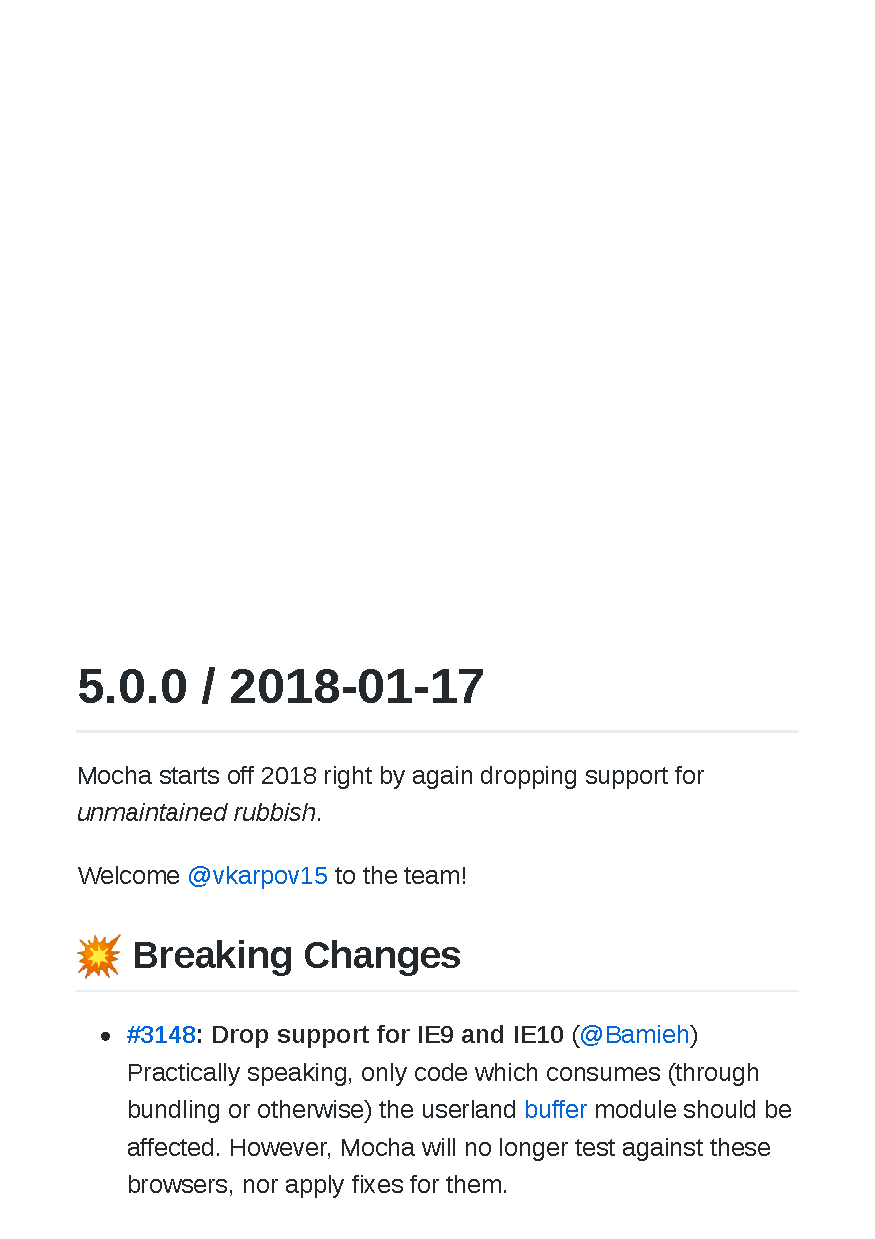
\includegraphics[scale=0.5]{figuras/bc_documentation_mocha.pdf}}\quad
        \subfigure[]{\label{fig:bc_documentation_other} 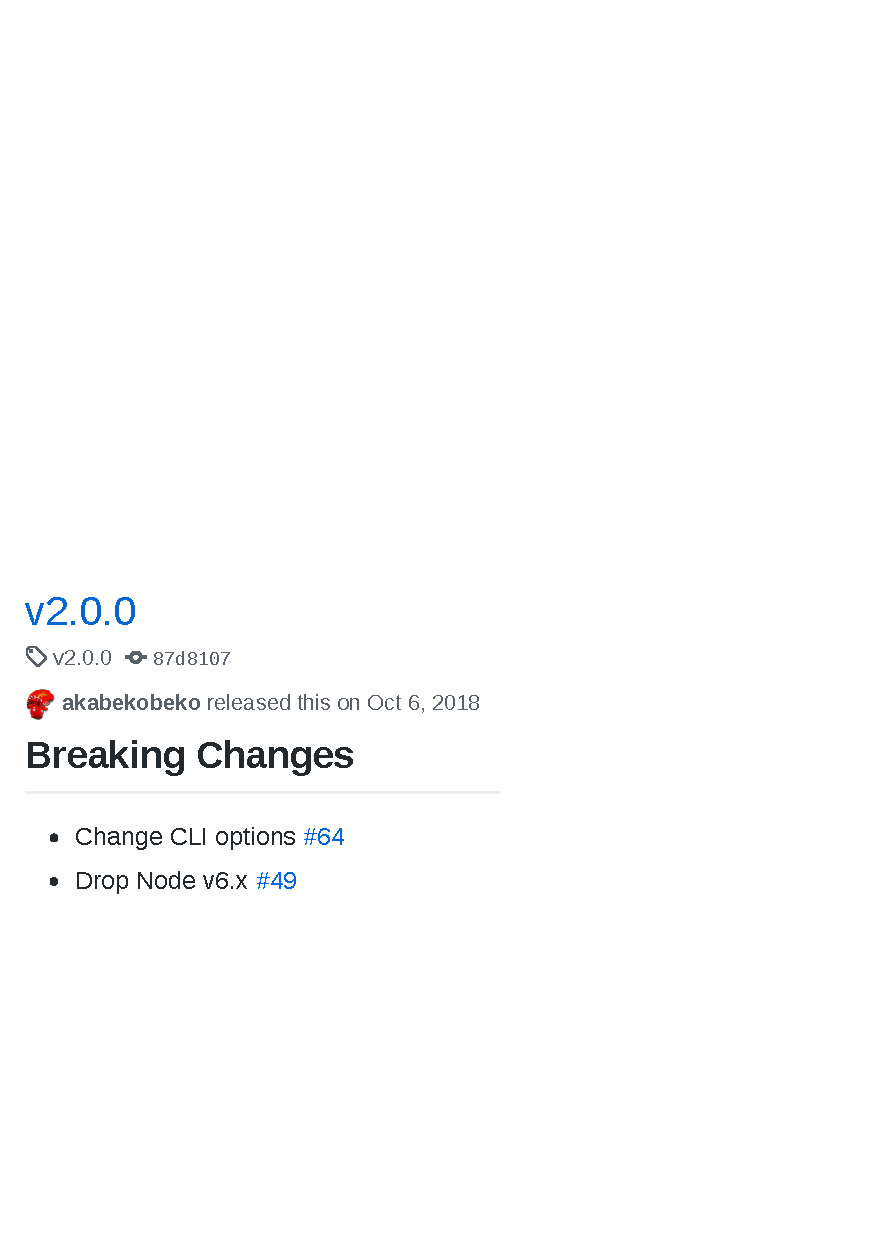
\includegraphics[scale=0.5]{figuras/bc_documentation_other.pdf}}
    }
    \caption{Exemplo de \textit{break changes} documentadas em \textit{changelogs} e \textit{relese-notes}}
    \label{fig:result_rq1_once_twice_three}
\end{figure}

Também buscamos em \textit{issues} e \textit{pull-requests} por comentários indicando as causas das \textit{breaking changes}. Após descobrir as alterações que introduziram as \textit{breaking changes}, foram analisadas e agrupadas cada uma dessas alterações em categorias mais genéricas possíveis. Por exemplo, todas as alterações relacionadas com mudança no tipo de variáveis foram agrupadas em uma categoria chamada \textit{Alteração de tipo de objeto}. Também foi analisado o nível do Versionamento Semântico em que a \textit{breaking change} foi introduzida pelo provedor e consertada pelo provedor ou cliente, bem como o local onde as \textit{breaking changes} foram documentadas (\textit{issues/pull-requests/changelogs}).

%---------------------------------------------------%
%----------------------RQ3--------------------------%
%---------------------------------------------------%

\subsubsection{\large QP3. Como os clientes se recuperam das \textit{breaking changes}?}
\label{sec:qp3}

% \subsubsection{Motivação:}
% \label{sec:qp3:motivation}
\textbf{Motivação:}
Uma \textit{breaking change} pode impactar um pacote cliente através de uma atualização \textit{implícita} ou \textit{explícita} de seu pacote provedor. Uma atualização implícita ocorre quando o cliente especificou o seu provedor como um \textit{range} de versões no \textit{package.json}. Então o \textsf{npm} descarrega automaticamente a nova \textit{release} do provedor. Já uma atualização explícita ocorre quando o cliente atualiza manualmente a versão do provedor no \textit{package.json} e o \textsf{npm} descarrega a nova versão especificada pelo cliente. Após uma \textit{breaking change}, o cliente pode se recuperar realizando uma alteração no seu código, aguardando uma nova \textit{release} do provedor que venha a consertar a \textit{breaking change} ou o cliente pode realizar um \textit{downgrade/upgrade} na versão do provedor.

As \textit{breaking changes} podem ser introduzidas pelo provedor \textit{direto} ou \textit{indireto}, uma vez que os clientes dependem de poucos provedores diretos mas dependem de muitos provedores indiretos \cite{npm-seven}. Mesmo quando o cliente tem poucos provedores diretos, muitos provedores indiretos podem propagar \textit{breaking changes}. Quando uma \textit{breaking change} se manifesta nos pacotes clientes, esses devem se recuperar uma vez que eles precisam executar sem erros e, também, eles podem ser provedores de outros pacotes nessa árvore de dependências. Portanto, uma \textit{breaking change} pode ser continuamente propagada enquanto não for consertada por nenhum dos pacotes. Até mesmo quando as \textit{breaking changes} podem ser consertadas atualizando-se para uma nova versão do provedor, os pacotes clientes precisam resolver manualmente as incompatibilidades que ainda existem \cite{Foo:2018:ESC:3236024.3275535}. Então, entender o comportamento da manifestação das \textit{breaking changes} pode ajudar os desenvolvedores a compreenderem quais são as maneiras mais efetivas e rápidas para se recuperar das \textit{breaking changes}.
\newline

% \subsubsection{Método:}
% \label{sec:qp3:approach}
\noindent
\textbf{Método:}
Todas as informações usadas para responder esta questão de pesquisa foram recuperadas dos repositórios dos pacotes clientes. Foram procuradas nesses repositórios informações sobre o erro e como os cliente se recuperaram da \textit{breaking change}. As seguintes informações foram analisadas:

\begin{itemize}
    \item \textbf{\textit{Commits:}} foram analisados manualmente os próximos \textit{commits} no repositório do cliente a partir da data da \textit{release} que contém a \textit{breaking change}. Foram analisados principalmente os \textit{commits} que alteraram o \textit{package.json} para verificar se o cliente realizou um \textit{downgrade/upgrade} ou se o cliente removeu ou substituiu o provedor.

    \item \textbf{\textit{Changelogs:}} o cliente pode mencionar nos \textit{changelogs} e nas \textit{release-notes} como foi realizada a recuperação da \textit{breaking change}, principalmente se o cliente realizou um \textit{downgrade/upgrade} na versão do provedor. Também, se o cliente consertou a \textit{breaking change} diretamente no seu código, provavelmente há essa informação nos \textit{changelogs}. Ao todo, 48\% dos repositórios dos clientes continham \textit{changelog} ou \textit{release-notes}.
    
    \item \textbf{\textit{Pull-requests/Issues:}} foram procurados \textit{pull-requests} e \textit{issues} no repositório do cliente que deveria consertar, ou conter informações sobre a \textit{breaking change}. \textit{Pull-requests/issues} nomeadas como \textit{Update provider}, \textit{Fix provider errors}, \textit{Fix tests} indicavam a presença de alguma alteração que foi realizada devido às \textit{breaking changes}.
\end{itemize}

Para cada caso de \textit{breaking change} foi recuperada a árvore de dependências do cliente até o provedor que introduziu a \textit{breaking change}. Por exemplo, em nosso segundo exemplo motivacional (Capítulo \ref{cap:exemplos}) foi recuperada a árvore de dependências a partir do cliente até \textsf{broccoli-asset-rev$\rightarrow$broccoli-filter$\rightarrow$broccoli-plugin} (Figura \ref{fig:dependency_tree}). Com isso foi analisada a quantidade de \textit{breaking changes} introduzida por provedores diretos e indiretos. 

Também foram investigados os dados sobre quando a \textit{breaking change} foi introduzida, consertada, qual pacote consertou e como foi realizada a correção. Assim foi analisado o tempo que as \textit{breaking changes} levaram para serem consertadas e quais são as principais maneiras como os clientes se recuperam das \textit{breaking changes}. Ainda foram analisados os casos onde o provedor consertou a \textit{breaking change} e, ainda assim, o cliente realizou um \textit{upgrade/downgrade} da versão do provedor. Por fim, foi verificado como as versões dos provedores foram alteradas pelos clientes e como a documentação da \textit{breaking change} influenciou na velocidade com que as \textit{breaking changes} foram consertadas.